\documentclass[12pt,a4paper]{article}

\usepackage{graphicx} % For adding images
\usepackage[a4paper, margin=1in]{geometry} % Page margins
\usepackage{setspace} % Line spacing
\usepackage{titlesec} % Section formatting
\usepackage{fancyhdr} % Footer
\usepackage{hyperref}

% Title Page
\title{\Huge \textbf{Final Project Report} \\ \vspace{0.5cm} \Large Image Processing Course}
\author{
    \Large \textbf{Team Members:} \\ 
    \large Fares Hazem \\ 
    \large Peter Hany \\ 
    \vspace{0.5cm} 
    \Large \textbf{Instructors:} \\ 
    \large Dr. Mahmoud Gamal \\ 
    \large Eng. Amany % Fixed line for Eng. Amany
}

\date{} % Remove default date

\begin{document}

% Title Page
\begin{titlepage}
    \centering
    % University logo
    
\includegraphics[width=0.3\textwidth]{university_logo.png} \\[1cm]
    
    % Title
    {\Huge \textbf{Final Project Report}} \\[0.5cm]
    {\Large Image Processing Course} \\[1cm]

    % Faculty and department
    {\Large \textbf{Faculty of Computers and Data Science}} \\[0.3cm]
    {\Large Department of Intelligent Systems} \\[1.5cm]

    % Author information
    {\Large \textbf{Team Members:}} \\[0.3cm]
    {\large Fares Hazem} \\ [0.3cm] 
    {\large Peter Hany} \\[1cm]
    
    % Instructor information
    {\Large \textbf{Instructors:}} \\[0.3cm]
    {\large Dr. Mahmoud Gamal} \\[0.3cm]  % Reduced space here
    {\large Eng. Amany} \\[1.5cm]  % Added \\
    
    % Footer
    {\Large Alexandria, Egypt} \\[0.3cm]
    {\large \textbf{Submission Date: 21 December 2024}} \\

    \vfill
    \rule{0.8\textwidth}{0.5pt} \\[0.2cm]
    {\small \textbf{Final Project for the Image Processing Course, 2024}}
\end{titlepage}




% Abstract Section
\newpage % Start a new page
\section*{\centering Abstract}

\setstretch{1.5} % Set line spacing for better readability

This project investigates the application of advanced image processing techniques, including \textbf{noise reduction}, \textbf{segmentation}, and \textbf{edge detection}, to solve real-world challenges across diverse domains. 

In the domain of \textit{autonomous vehicles}, the focus is on \textbf{lane detection} in road images, leveraging datasets such as \textit{Carla}. By applying robust algorithms, we aimed to enhance image quality, identify critical regions of interest, and extract meaningful features.

This report delves into the methods, parameters, and challenges encountered throughout the project. It also highlights the solutions implemented and the insights gained, underscoring the transformative potential of image processing in these vital applications.

\vspace{0.5cm}
\noindent \textbf{Keywords:} Image Processing, Noise Reduction, Segmentation, Edge Detection, Autonomous Vehicles, Lane Detection

\newpage % Start a new page
\section{Introduction}

\setstretch{1.5} % Set line spacing for better readability

Lane detection is a crucial component of autonomous driving systems, enabling vehicles to safely navigate roads by identifying and following lane markings. As self-driving technology continues to evolve, accurate lane detection is vital for ensuring safety and efficiency on the road.

This project explores the application of various image processing techniques to solve the challenge of lane detection in road images. Specifically, we apply multiple methods to detect road lanes, including:
\begin{itemize}
    \item \textbf{Noise Reduction:} Eliminating unwanted disturbances to improve image clarity and accuracy.
    \item \textbf{Segmentation:} Isolating lane markings from the surrounding environment for better detection.
    \item \textbf{Edge Detection:} Identifying boundaries of lane markings using techniques like Canny edge detection.
\end{itemize}

The dataset used for this project comes from \textit{Carla}, a well-known simulation platform for autonomous driving research. We aim to demonstrate how combining these techniques can enhance lane detection performance in varied road conditions.

\vspace{0.5cm}
\noindent \textbf{Report Structure:} 
This report is organized as follows:
\begin{enumerate}
    \item \textbf{Methodology:} Describes the techniques used for lane detection, including noise reduction, segmentation, and edge detection.
    \item \textbf{Results and Discussion:} Analysis of the lane detection results and evaluation of the techniques' effectiveness.
    \item \textbf{Conclusion and Future Work:} Summary of findings and suggestions for improving lane detection systems.
\end{enumerate}




\newpage % Start a new page
\section{Methodology}

\setstretch{1.5} % Set line spacing for better readability

\subsection{Noise Reduction}

Noise reduction is a crucial step in preparing images for further processing. We applied various techniques to reduce noise while preserving important image features. The following filters were used:

\vspace{1em} % Adds some vertical space between titles
\textbf{Mean (Average) Filter}

\begin{figure}[h!]
    \centering
    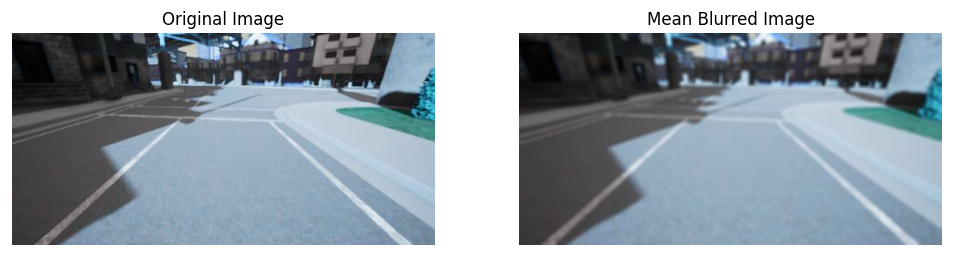
\includegraphics[width=1.05\textwidth]{mean_filter.png} % Adjusted size to fit page
    \caption{Mean Filter Result.}
    \label{fig:mean_filter}
\end{figure}

\vspace{1em} % Adds some vertical space between titles
\textbf{Median Filter}\textit {(Best Result)}

\begin{figure}[h!]
    \centering
    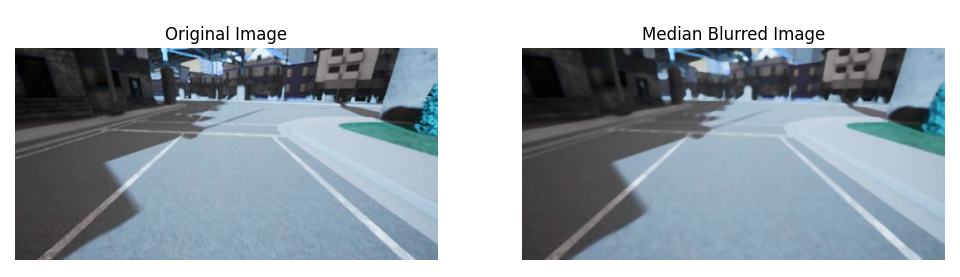
\includegraphics[width=1.05\textwidth]{median_filter.png} % Adjusted size to fit page
    \caption{Median Filter Result (Best Result).}
    \label{fig:median_filter}
\end{figure}




\newpage % Start a new page for the next content

\vspace{1em} % Adds some vertical space between titles
\textbf{Maximum Filter}

\begin{figure}[h!]
    \centering
    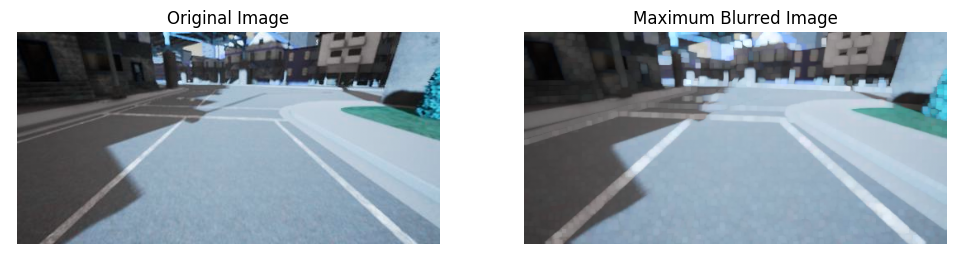
\includegraphics[width=1.05\textwidth]{maximum_filter.png} % Adjusted size to fit page
    \caption{Maximum Filter Result.}
    \label{fig:maximum_filter}
\end{figure}

\vspace{1em} % Adds some vertical space between titles
\textbf{Minimum Filter}

\begin{figure}[h!]
    \centering
    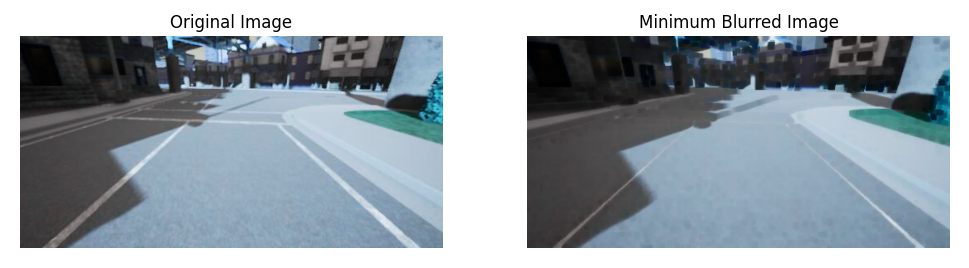
\includegraphics[width=1.05\textwidth]{minimum_filter.png} % Adjusted size to fit page
    \caption{Minimum Filter Result.}
    \label{fig:minimum_filter}
\end{figure}

\vspace{1em} % Adds some vertical space between titles
\textbf{Gaussian Blur Filter}

\begin{figure}[h!]
    \centering
    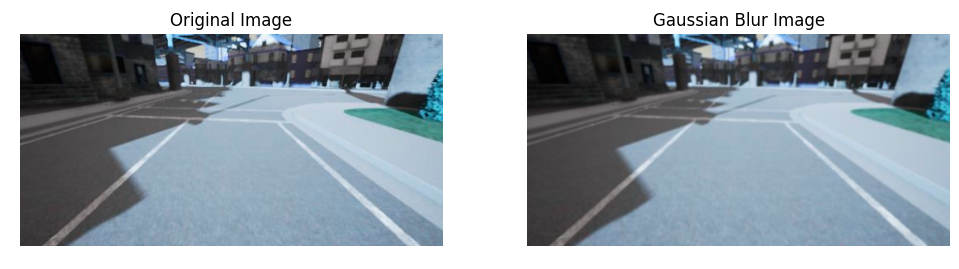
\includegraphics[width=1.05\textwidth]{gaussian_blur.png} % Adjusted size to fit page
    \caption{Gaussian Blur Filter Result.}
    \label{fig:gaussian_blur}
\end{figure}

After visualizing the results, the \textbf{Median Filter} was found to provide the best results, effectively reducing noise while preserving lane markings.




\newpage % Start a new page

\subsection{Contrast Enhancement}

Contrast enhancement is essential for improving the visibility of important features in images. Two techniques were applied to enhance the contrast:

\vspace{1em} % Adds some vertical space between titles
 \textbf{Linear Contrast Stretching} \textit{(Best Result)}

\begin{figure}[h!]
    \centering
    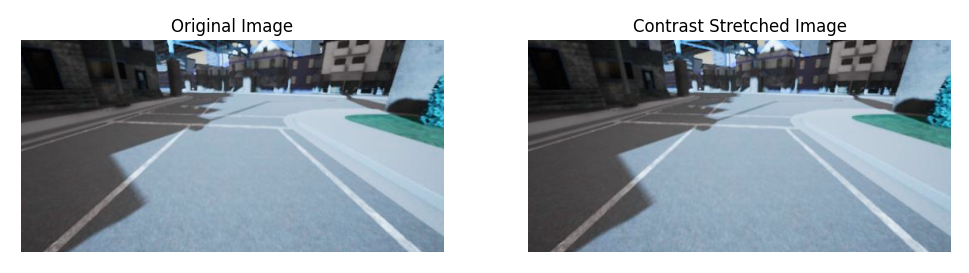
\includegraphics[width=1.05\textwidth]{linear_contrast_stretching.png} % Adjusted size to fit page
    \caption{Linear Contrast Stretching Result (\textit{Best Result}).}
    \label{fig:linear_contrast_stretching}
\end{figure}

\vspace{1em} % Adds some vertical space between titles
\textbf{Histogram Equalization}

\begin{figure}[h!]
    \centering
    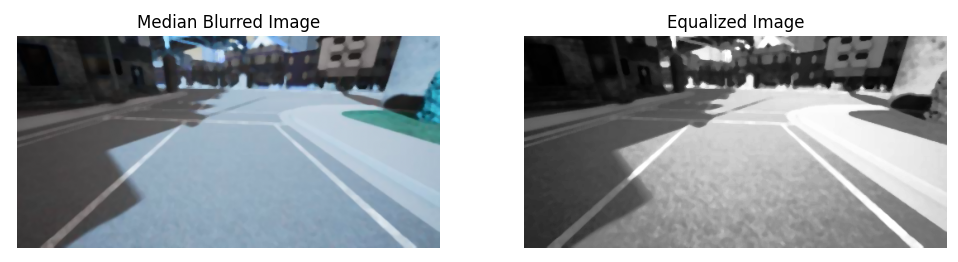
\includegraphics[width=1.05\textwidth]{histogram_equalization.png} % Adjusted size to fit page
    \caption{Histogram Equalization Result.}
    \label{fig:histogram_equalization}
\end{figure}

After visualizing the results, it was found that \textit{Linear Contrast Stretching} provided the best results for lane visibility.

\newpage % Start a new page

\subsection{Image Segmentation}

Image segmentation is crucial for separating relevant features from the background. We tested several thresholding and region-based methods:

\begin{itemize}
    \item \textbf{Histogram-Based Methods}
    \item \textbf{Region-Based Methods} 
\end{itemize}

\subsubsection*{\textbf{Histogram-Based Methods}}

\vspace{0.5em} % Adds some vertical space between titles
\hspace{1em} \textbf{Simple Thresholding} \textit{(Intermediate Result)}


\begin{figure}[h!]
    \centering
    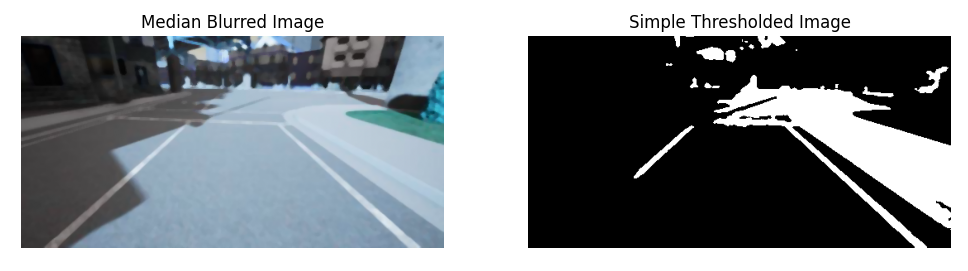
\includegraphics[width=1.05\textwidth]{simple_thresholding.png}
    \caption{Simple Thresholding Result.}
    \label{fig:simple_thresholding}
\end{figure}

\vspace{0.5em} % Adds some vertical space between titles
 \textbf{Global Thresholding }\textit{(Bad Result)}

\begin{figure}[h!]
    \centering
    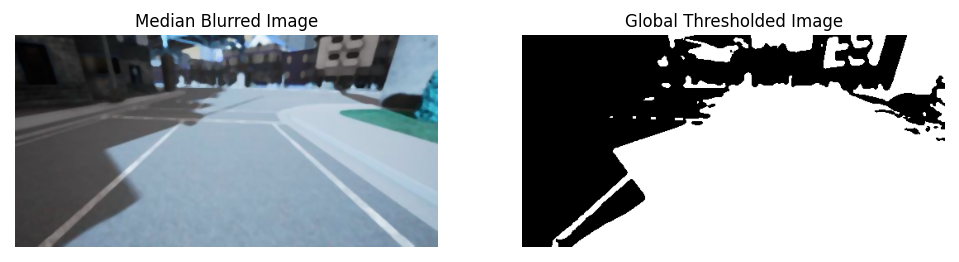
\includegraphics[width=1.05\textwidth]{global_thresholding.png}
    \caption{Global Thresholding Result (\textit{Bad Result}).}
    \label{fig:global_thresholding}
\end{figure}

\newpage % Start a new page

\vspace{0.5em} % Adds some vertical space between titles
 \textbf{Adaptive Thresholding} \textit{(Intermediate Result)}

\begin{figure}[h!]
    \centering
    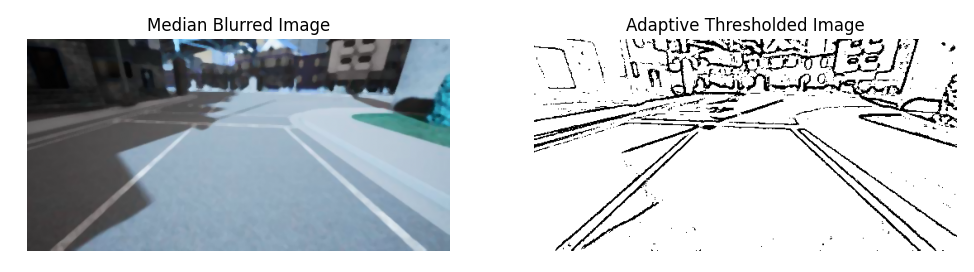
\includegraphics[width=1.05\textwidth]{adaptive_thresholding.png}
    \caption{Adaptive Thresholding Result (\textit{Intermediate Result}).}
    \label{fig:adaptive_thresholding}
\end{figure}

\vspace{0.5em} % Adds some vertical space between titles
 \textbf{Otsu Thresholding} \textit{(Bad Result)}

\begin{figure}[h!]
    \centering
    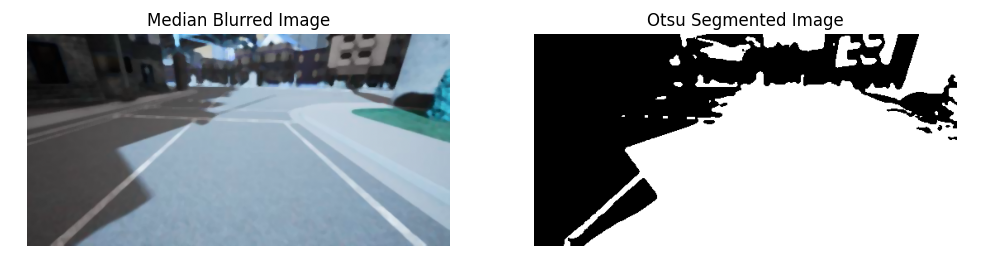
\includegraphics[width=1.05\textwidth]{otsu_thresholding.png}
    \caption{Otsu Thresholding Result (\textit{Bad Result}).}
    \label{fig:otsu_thresholding}
\end{figure}

\newpage % Start a new page

\subsubsection*{Region-Based Methods}

\vspace{0.5em} % Adds some vertical space between titles
\hspace{1em}\textbf{Clustering} \textit{(Bad Result)}

\begin{figure}[h!]
    \centering
    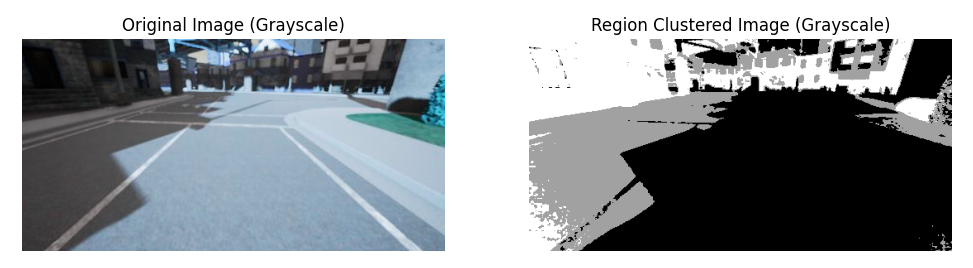
\includegraphics[width=1.05\textwidth]{clustering.png}
    \caption{Clustering Result (\textit{Bad Result}).}
    \label{fig:clustering}
\end{figure}

\vspace{0.5em} % Adds some vertical space between titles
\textbf{Growth Region} \textit{(Bad Result, Needs Optimization)}

\begin{figure}[h!]
    \centering
    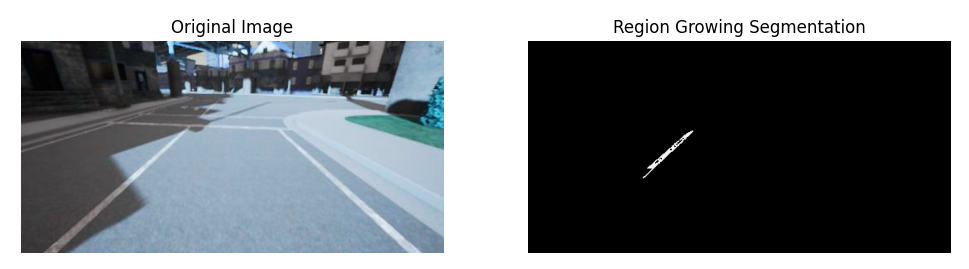
\includegraphics[width=1.05\textwidth]{growth_region.png}
    \caption{Growth Region Result (\textit{Needs Optimization}).}
    \label{fig:growth_region}
\end{figure}

\vspace{0.5em} % Adds some vertical space between titles
\textbf{Split \& Merge} \textit{(Bad Result, Needs Optimization)}

\begin{figure}[h!]
    \centering
    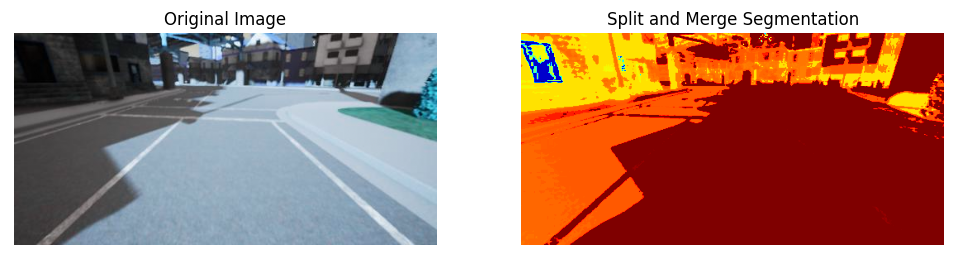
\includegraphics[width=1.05\textwidth]{split_merge.png}
    \caption{Split \& Merge Result (\textit{Needs Optimization}).}
    \label{fig:split_merge}
\end{figure}





\subsection{Edge Detection}

Edge detection is essential for detecting lane boundaries and other important features. We compared several methods:

\vspace{0.5em} % Adds some vertical space between titles
\textbf{Sobel Filter} \textit{(Intermediate Result)}

\begin{figure}[h!]
    \centering
    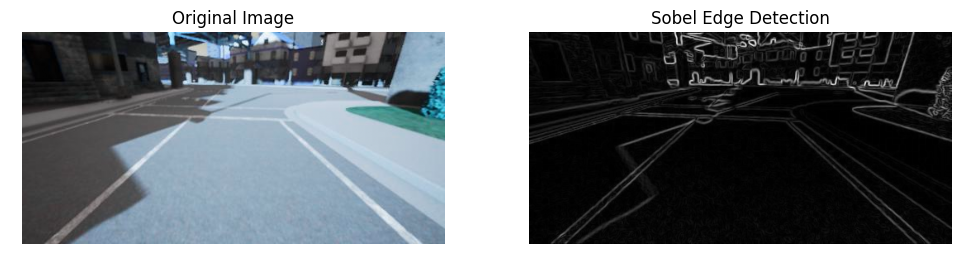
\includegraphics[width=1.05\textwidth]{sobel_filter.png}
    \caption{Sobel Filter Result.}
    \label{fig:sobel_filter}
\end{figure}

\vspace{0.5em} % Adds some vertical space between titles
\textbf{Prewitt Filter} \textit{(Intermediate Result but Very Noisy Image)}

\begin{figure}[h!]
    \centering
    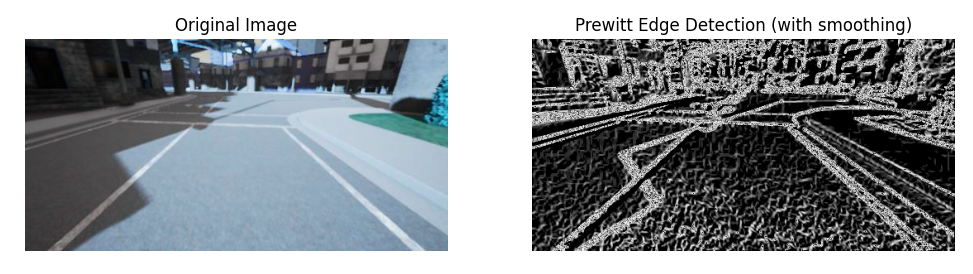
\includegraphics[width=1.05\textwidth]{prewitt_filter.png}
    \caption{Prewitt Filter Result (Very Noisy Image).}
    \label{fig:prewitt_filter}
\end{figure}

\textbf{Canny Edge Detection with Morphological Operations} \textit{(Best Result)}

\begin{figure}[h!]
    \centering
    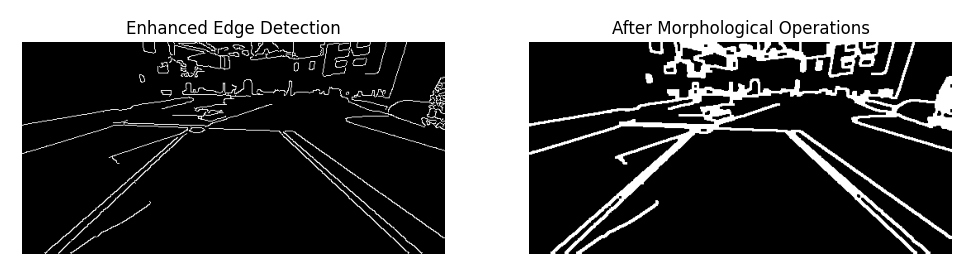
\includegraphics[width=1.05\textwidth]{canny_edge_detection.png}
    \caption{Canny Edge Detection with Morphological Operations (Best Result).}
    \label{fig:canny_edge_detection}
\end{figure}




\newpage % Start a new page

\section{Final Lane Detection Results}

The final lane detection results were achieved by combining noise reduction, contrast enhancement, segmentation, and edge detection. Below are the images showing the original image with keypoints, birdseye image, and thresholded output.

\begin{figure}[h!]
    % Title before the figure
    \subsection*{On Carla Dataset:}

    % First image (HSV Thresholding) on top
    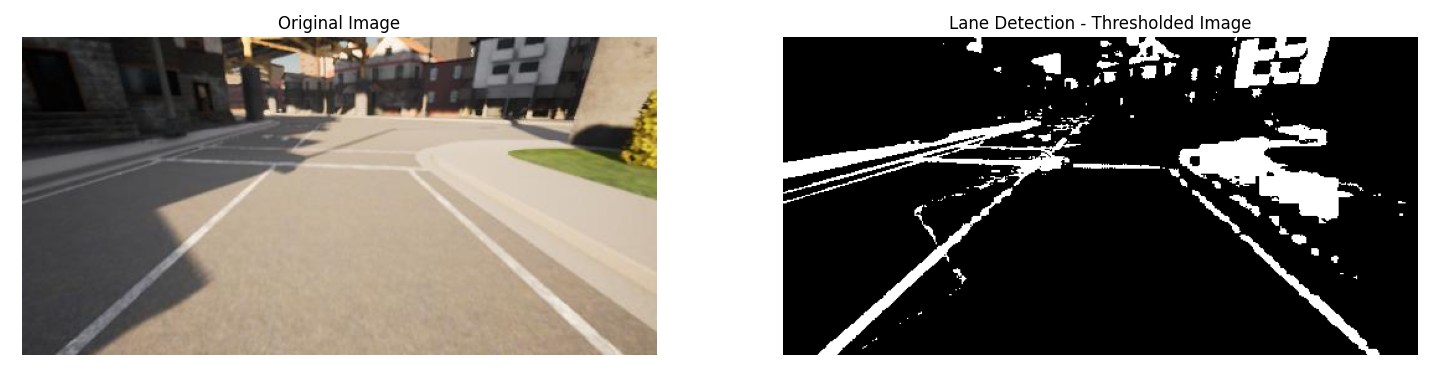
\includegraphics[width=1.05\textwidth]{hsv_thresholding.png}
    \caption{HSV Thresholding Result.}
    \label{fig:hsv_thresholding}
\end{figure}

\begin{figure}[h!]
    % Title before the figure
    \subsection*{On Video Found Online:}
    \centering
    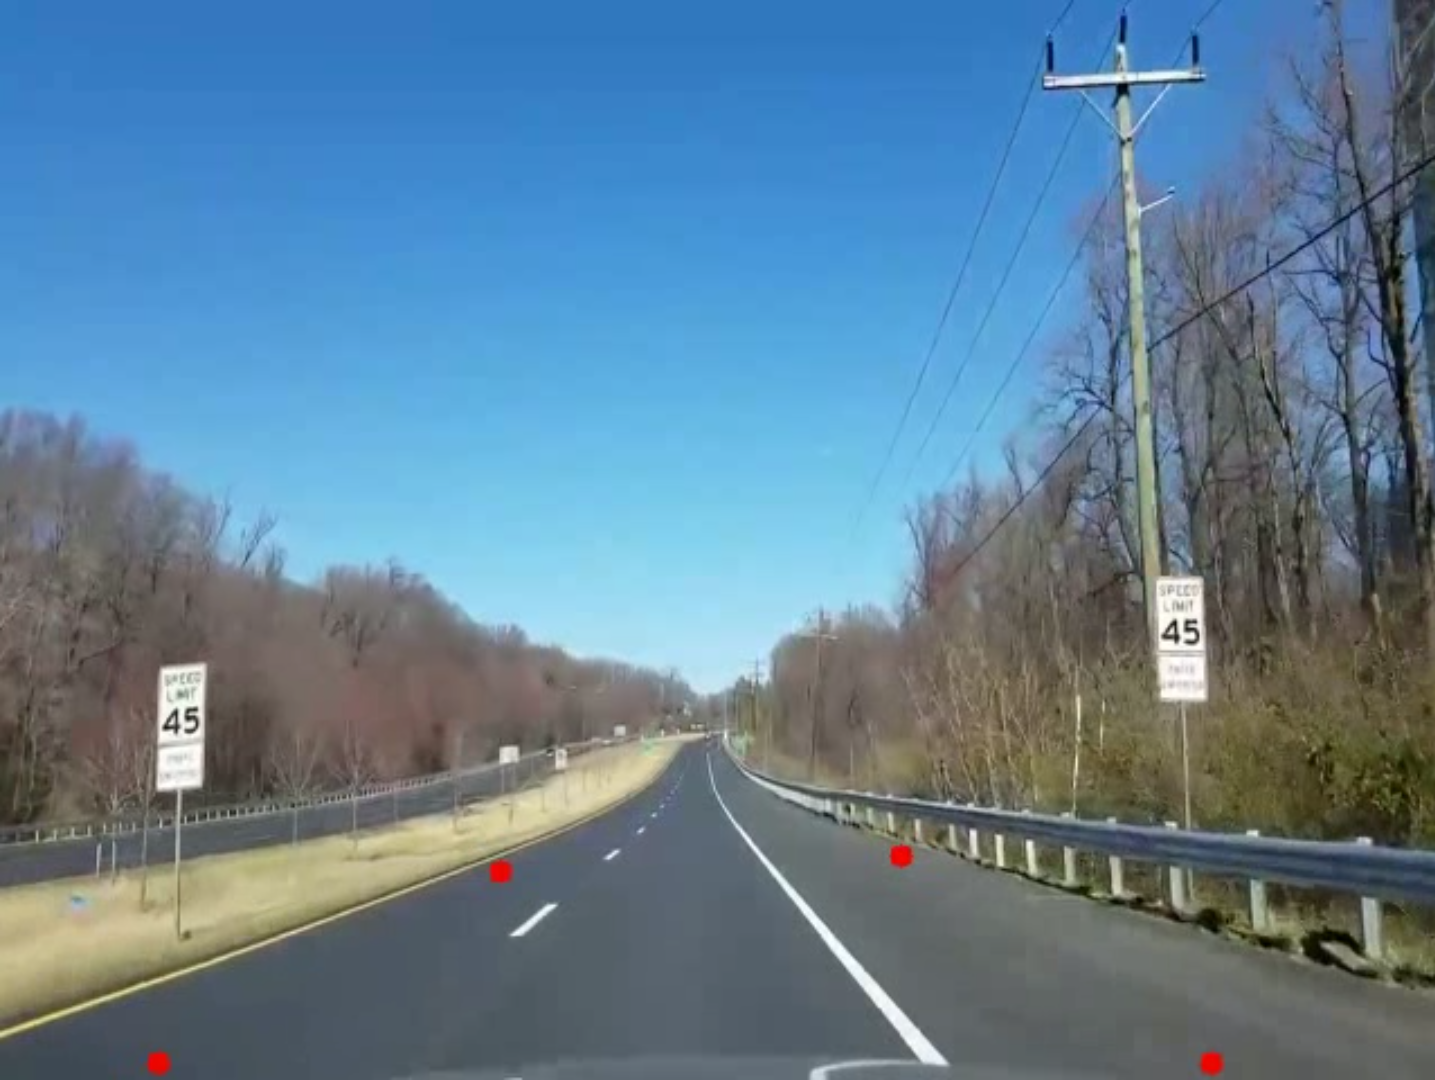
\includegraphics[width=0.40\textwidth]{original_image_with_keypoints.png}
    
    \vspace{0.5em} % Increases vertical space between images
    
    % Second row with two images side by side
    \begin{minipage}{0.40\textwidth}
        \centering
        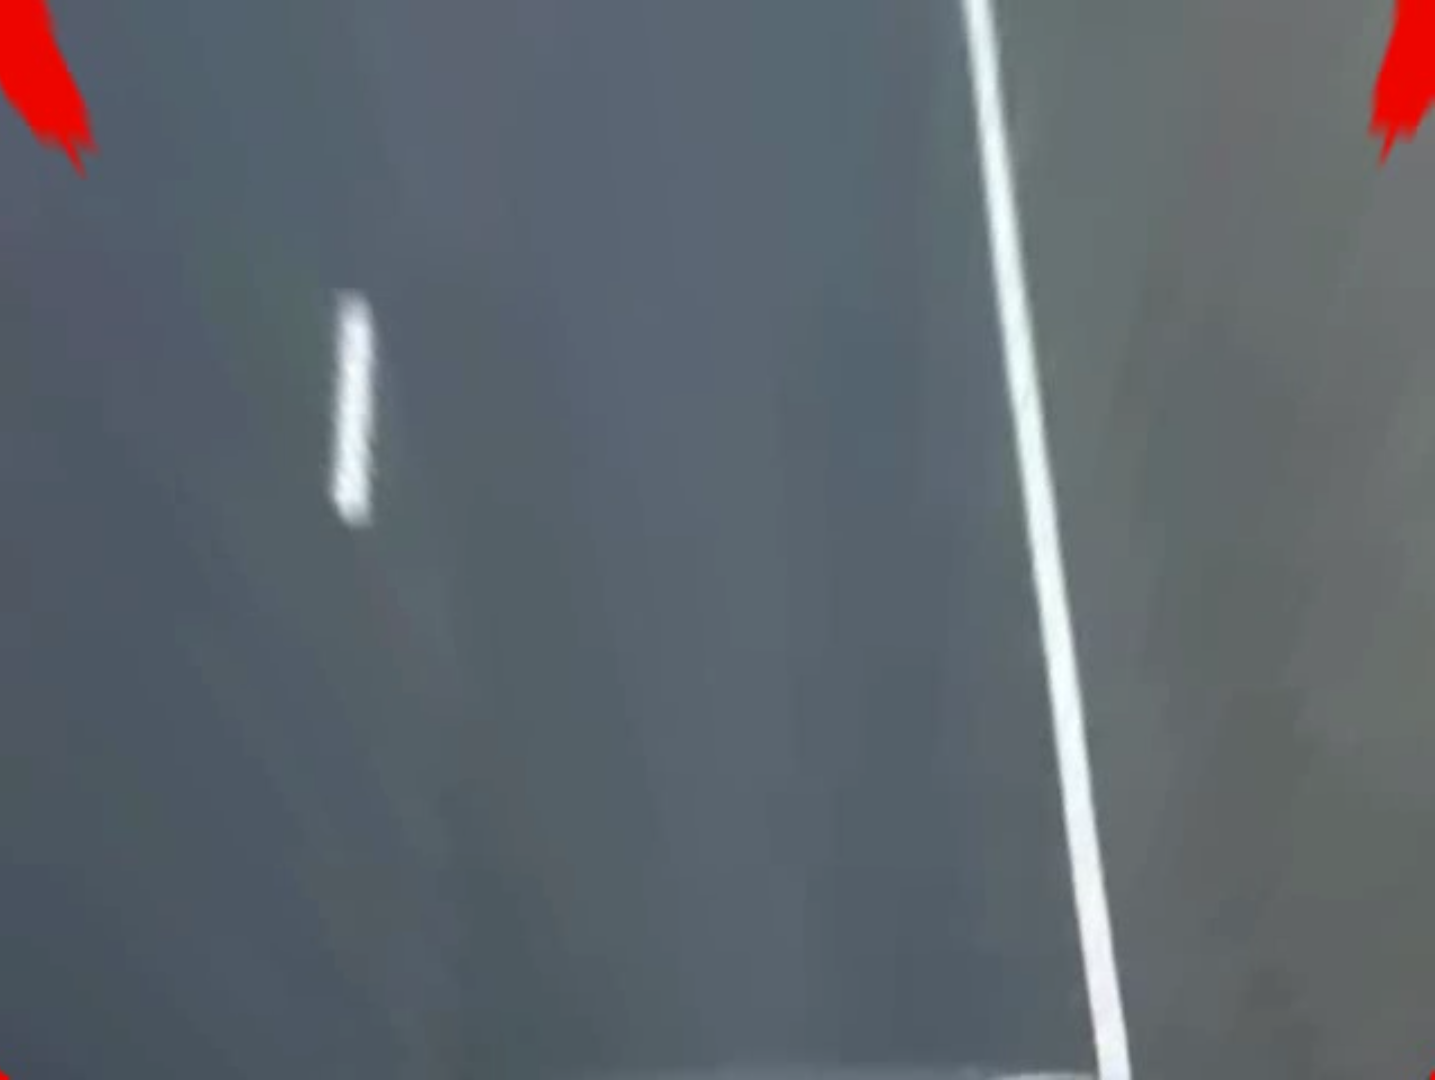
\includegraphics[width=\textwidth]{birdseye_image.png}
    \end{minipage}% 
    \hspace{0.5em} % Adds horizontal space between the images
    \begin{minipage}{0.40\textwidth}
        \centering
        
\includegraphics[width=\textwidth]{thresholded_output.png}
    \end{minipage}

    % Title after the figure
    \vspace{0.5em} % Adds space between the figure and title

    \caption{Lane Detection Results: Comparison of HSV Thresholding, Original Image with Keypoints, Birdseye Image, and Thresholded Output.}
    \label{fig:lane_detection}
\end{figure}



\newpage % Start a new page

\section{Discussion}

\begin{itemize}
    \item \textbf{Challenges faced:} 
    \begin{itemize}
        \item Image processing techniques are quite \textbf{old} and \textbf{hard to apply} because they require careful \textbf{selection}, \textbf{tuning}, and \textbf{optimization} of parameters to achieve the best results. This process can be \textbf{time-consuming}.
        \item \textbf{Lighting issues} in the dataset made the processing more difficult, especially when applying filters to the images. A \textbf{cleaner dataset} would have been preferable for better results.
    \end{itemize}
    \item \textbf{Solution applied:} We focused on \textbf{HSV Thresholding}, which proved to be more efficient than the traditional methods. \textbf{Tuning} the parameters for HSV is simpler and faster.
    \item \textbf{Analysis of results:} The \textbf{HSV Thresholding method} provided a \textbf{better result}, especially when compared to other image processing methods that require more complex fine-tuning.
\end{itemize}

\section{Conclusion and Future Work}

\begin{itemize}
    \item \textbf{Summary of findings:} 
    \begin{itemize}
        \item The image processing techniques used, though effective, require a lot of \textbf{manual tuning} and can be \textbf{time-consuming}.
        \item \textbf{HSV Thresholding} emerged as a more \textbf{efficient} and \textbf{easier-to-tune} method, giving more consistent results with less effort.
    \end{itemize}
    \item \textbf{Suggestions for future work:}
    \begin{itemize}
        \item The use of \textbf{AI} could lead to more \textbf{consistent} and \textbf{generalized results} across different datasets and lighting conditions.
        \item Once the best solution is found, it should be \textbf{applied to the entire dataset} to improve accuracy and reliability.
    \end{itemize}
\end{itemize}

\section{References}

\begin{itemize}
    \item \textbf{Cited works:}  
    \begin{itemize}
        \item Aditya Singh's lane detection project on GitHub: 
        \href{https://github.com/Aditya-Singh-SSJ2/Lane_Detection_Sliding_Windows/tree/main}{https://github.com/Aditya-Singh-SSJ2/Lane\_Detection\_Sliding\_Windows/tree/main}
    \end{itemize}
    \item \textbf{Dataset:}  
    \begin{itemize}
        \item Lane Line Detection Dataset (Kaggle): \url{https://www.kaggle.com/datasets/hyunkunkookminuniv/lanelinedetection}
    \end{itemize}
\end{itemize}

\end{document}
